\section{Durchführung}
\label{sec:Durchführung}

\subsection{Versuchsaufbau}
\label{sec:Versuchsaufbau}
%\begin{figure}
%	\centering
%	\caption{Schematische Darstellung des Versuchsaufbaus \cite{anleitung}.}
%	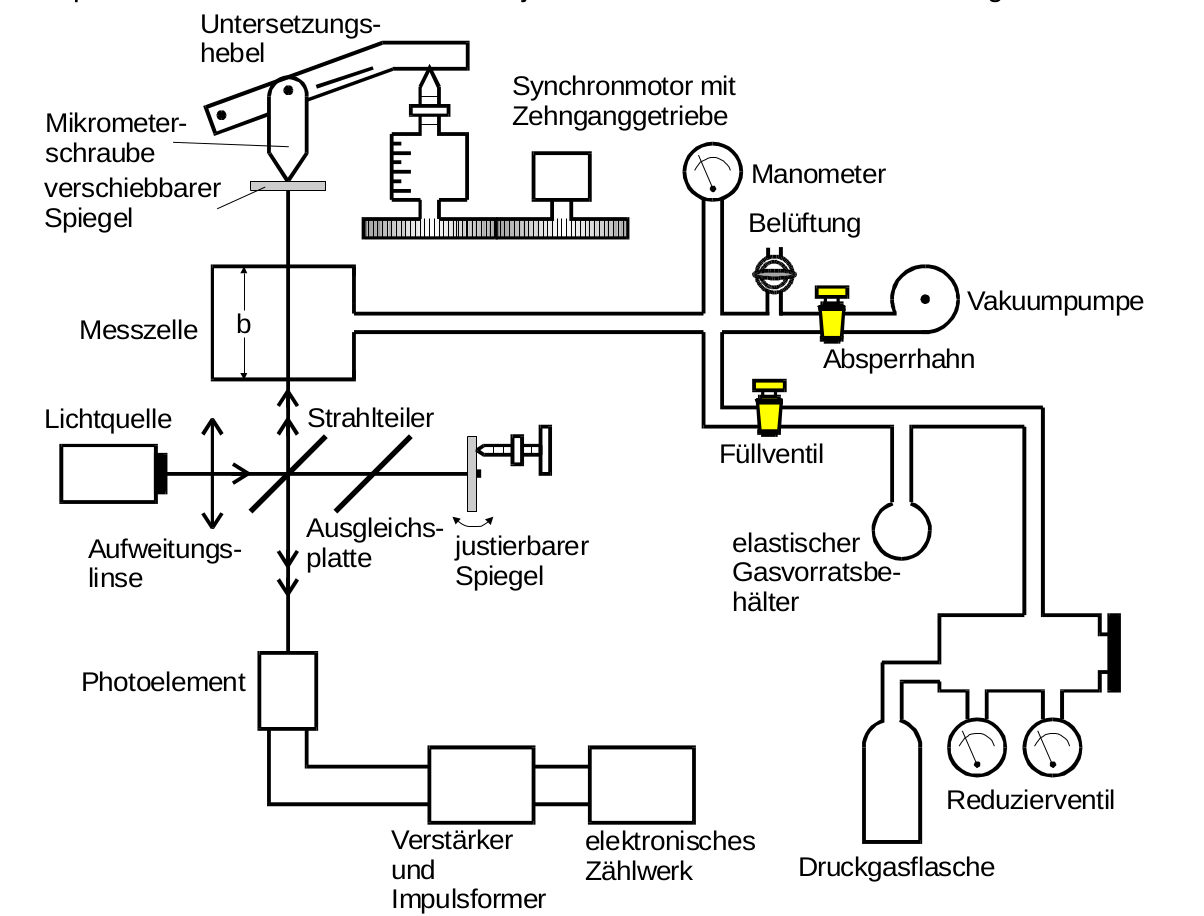
\includegraphics{Bilder/aufbau.png}
%	\label{fig:aufbau}
%\end{figure}
%
%\begin{figure}
%	\centering
%	\caption{Schematische Darstellung der Quelle zur Erzeugung radioaktiven Isotopen \cite{anleitung}.}
%	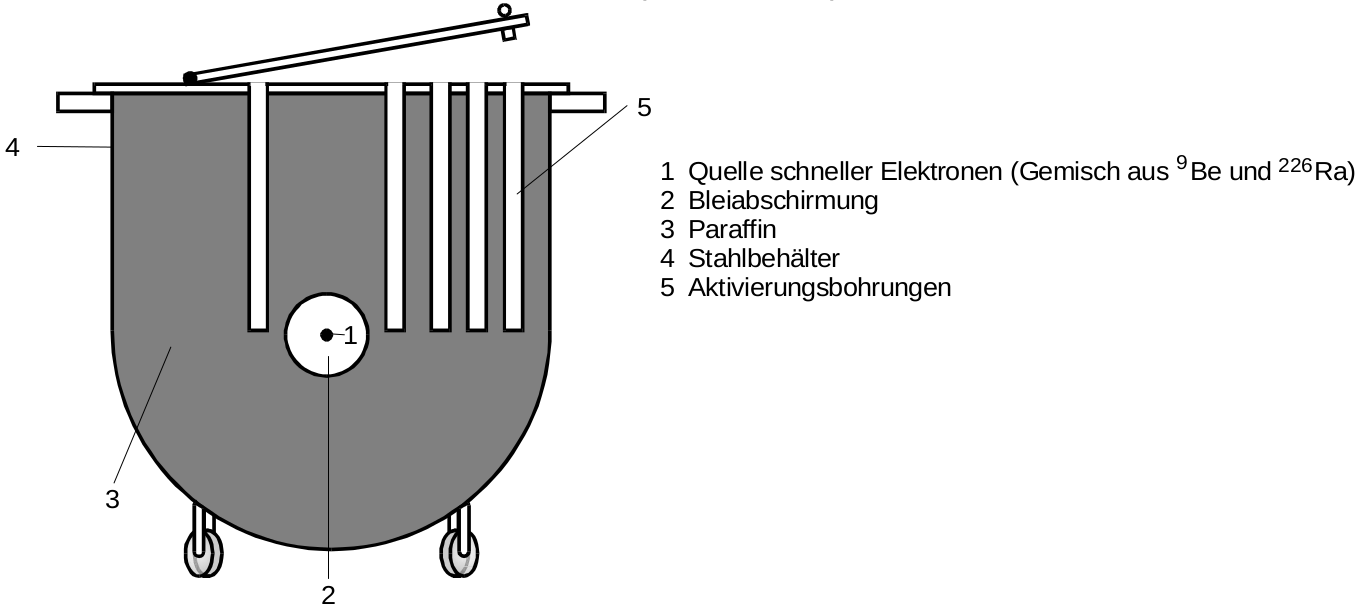
\includegraphics{content/toepfchen.png}
%	\label{fig:kochen}
%\end{figure}
%
Der Versuchsaufbau -- wie in Abbildung \ref{fig:aufbau} dargestellt -- besteht im Wesentlichen 
aus einem zerfallenden radioaktiven Isotop und einem Geiger-Müller-Zählrohr, welches die 
zerfallenden Kerne misst.
Das Geiger-Müller-Zählrohr ist entspricht einer mit Gas gefüllten Röhre. Trifft ein $\beta$-
oder $\gamma$- Teilchen auf ein Gasteilchen wird dieses ionisiert und kann aufgrund einer
anliegenden Spannung an der Röhre gemessen werden.
Dabei werden die gemessenen Zerfälle pro Messzeitintervall, welches am Zeitgeber einstellbar 
ist, an den Zählern 1 und 2 angezeigt. Nach jedem Messvorgang wird der Zähler umgeschaltet und 
der vorherige Wert auf dem aktuellen Zähler wird überschrieben. Der Versuchsaufbau ist mit
einer Blei-Abschirmung ausgestattet um die radioaktive Strahlung abzuschirmen.

Zur Erzeugung der radioaktiven Isotope wird das Objekt in Abbildung \ref{fig:kochen} verwendet.
Hierbei werden stabile Kerne mit niederenergetischen Neutronen beschossen. 
Da die Neutronen ihre Energie durch elastische Stöße an die Kerne übergeben und die maximale
Energie bei gleichen Massen der Stoßpartner erreicht wird, werden die Neutronen in einem 
Paraffinmantel gebremst, bis sie die optimale Energie besitzen.


\subsection{Versuchsbeschreibung}
\label{sec:Versuchsbeschreibung}
Zu Beginn des Versuchs muss das Michelson-Interferometer für die Messung justiert werden.
Dazu wird der Laser eingeschaltet und an die Position des Photoelements (vgl. Abbildung \ref{fig:aufbau}) eine Mattscheibe eingebracht.\\
Der justierbare Spiegel wird so ausgerichtet, dass die beiden hellsten Intensitätsmaxima der beiden ankommenden Strahlen möglichst genau zur Deckung gebracht werden. Das Photoelement wird entsprechend so ausgerichtet, dass das Intensitätsmaxima beider Strahlen genau auf den Eintrittsspalt des Photoelements liegt.
\\Für die Messung der Wellenlänge des Lasers wird der verschiebbare Spiegel genutzt.
Dazu wird der Synchronmotor eingeschaltet und eine Verschieberichtung ausgewählt.
Zu beachten ist hierbei, dass der Motor nicht zu schnell bewegt wird, da sonst das Photoelement nicht alle ankommenden konstruktiven Interferenzen, also Intensitätsmaxima der ankommenden Strahlen, als getrennte Intensitätsmaxima eindeutig zählen kann und somit das falsche Ergebnis liefert.
\\Bei Bedarf muss ein kleinerer Gang ausgewählt werden. Im vorliegenden Experiment wurde die Messung im kleinsten Gang durchgeführt.
Nachdem etwa 1000 konstruktive Interferenzen der Teilstrahlen am Photoelement registriert wurden, wird die exakte Anzahl an registrierten Interferenzen notiert sowie die Verschiebestrecke des Spiegels über die Verschiebung der Mikrometerschraube bestimmt. Dazu wird die Position zu Beginn und zum Ende der Verschiebung an der Mikrometerschraube abgelesen und mittels der Hebelübersetzung die Verschiebestrecke $\Delta d$ berechnet.
\\Die Messung wird etwa sieben- bis zehnmal durchgeführt.

Zur Bestimmung des Brechungsindex von Luft wird der verschiebbare Spiegel nicht mehr bewegt.\\
Die Messzelle wird mittels der Vakuumpumpe auf den Druck $p$ evakuiert, welcher notiert wird. Beim langsamen Wiedereinlassen der Luft werden erneut die konstruktiven Interferenzen am Photoelement gezählt und sobald wieder der Normaldruck $p_{\mathrm{0}}$ in der Messzelle herrscht, wird deren Anzahl $z$ notiert. \\Die Messung wird sieben-bis zehnmal wiederholt.

Für die Messung des Brechungsindex von $\mathrm{CO_2}$ wird die Messzelle evakuiert und der Druck $p$ notiert.\\
Es wird langsam $\mathrm{CO_2}$ in die Messzelle strömen gelassen und erneut die Anzahl an beobachteten Intensitätsmaxima $z$ notiert sobald in der Messzelle wieder der Normaldruck $p_0$ vorliegt.
\\Da sich noch Luftrückstände in der Messzelle befinden könnten, wird die Messung ebenso etwa sieben-bis zehnmal wiederholt.
